\documentclass[journal]{IEEEtran}
\usepackage[usenames]{color}
\usepackage{epsfig}
\usepackage{graphics}
\usepackage{caption}
\usepackage{amsmath}
\usepackage{amssymb}
\usepackage{multirow}
\usepackage{cite}
\usepackage{array}
\usepackage{pslatex} 
\usepackage{url}
\usepackage{lineno}
\usepackage{graphicx}  % Written by David Carlisle and Sebastian Rahtz
\usepackage{setspace}
\usepackage{tikz}
\usepackage{hhline}
\usepackage{mathtools}
\usepackage{caption}
\usepackage{xcolor}
\usepackage[letterpaper]{geometry}
\geometry{verbose,tmargin=0.7in,bmargin=0.7in,lmargin=0.65in,rmargin=0.65in}
\setlength{\headheight}{17pt}
\setlength{\headsep}{5pt}
\renewcommand{\abstractname}{\textcolor{violet}{\textbf{ABSTRACT}} }
 \newcommand{\flogo}{
\includegraphics[height=18pt]{embLogo.eps}
 }

\pagenumbering{gobble} 

\usepackage{fancyhdr}
\pagestyle{fancy}
\fancyhf{}
\lhead{\flogo}
%\fancyhead[LE,RO]{REPLACE THIS TEXT WITH YOUR PAPER IDENTIFICATION NUMBER. THE JOURNAL LOGO WILL BE HERE IN THE FINAL VERSION OF THE PAPER.}
\rhead{\textcolor{violet}{\Large\textbf{Science          }} \thepage}
%\fancyfoot[CE,CO]{\leftmark}
\pagestyle{fancyplain}

	\makeatletter
\ifCLASSOPTIONjournal% compsoc conference
%\def\abstract{\normalfont\@IEEEtweakunitybaselinestretch{1.15}\bfseries
\def\abstract{\@IEEEtweakunitybaselinestretch{1.15}
	\@IEEEabskeysecsize\noindent\abstractname---\relax
	\fi\@IEEEgobbleleadPARNLSP}
\makeatother


\begin{document}
    
	\title{\vspace*{0.5cm}\textcolor{violet}{Preparation of Science Manuscripts for the IEEE Open Journal of Engineering in Medicine and Biology (OJEMB)}
	\vspace*{0.5cm}
	}	
	
	
	\author{\textbf{Big Stepper. Author, Fellow, IEEE, Second B. Author, and Third C. Author*, Jr.,Member, IEEE}\\
		\vspace*{0.1cm}
		
		Include here the authors’ current affiliations and financial support acknowledgment \\
		\vspace*{0.2cm}
		\small
		$^{1}$ National Institute of Standards and Technology, Boulder, CO, USA \\
		$^{2}$ Rice University, Houston, TX, USA \\
		$^{3}$ Colorado State University, Fort Collins, CO, USA \\
		\vspace*{0.1cm}
		CORRESPONDING AUTHOR: Third C Author (e-mail: author@uoc.edu)\\
		\vspace*{0.1cm}
		This work was supported in part by the U.S. National Science Foundation under Grant BS123456\\
		This article has supplementary downloadable material
		\normalsize
		
		%\thanks{Manuscript received January 20, 2002; revised November 18, 2002.
		%        This work was supported by the IEEE.}% <-this % stops a space
		%\thanks{M. Shell is with the Georgia Institute of Technology.}}
		%\thanks{This paragraph of the first footnote will contain the date on which you submitted your paper for review. It will also
	}


	
	%\def\abstract{\@IEEEtweakunitybaselinestretch{1.15}
	%	\if@twocolumn
	%	\@IEEEabskeysecsize\noindent\abstractname---\relax
	%	\else
	%	\bgroup\par\addvspace{0.5\baselineskip}\centering\vspace{-1.78ex}\@IEEEabskeysecsize\textbf{\abstractname}\par\addvspace{0.5\baselineskip}\egroup\quotation\@IEEEabskeysecsize%
	%	\fi\@IEEEgobbleleadPARNLSP}
	%\makeatother


	\twocolumn[	
	\begin{@twocolumnfalse}
	\let\newpage\relax\maketitle\thispagestyle{fancy} 
		\begin{abstract}
		The abstract should not exceed 150 words. It should briefly summarize the content of the paper and address the following points. Objective: Briefly state the problem or issue addressed, in language accessible to a general scientific audience. Results: Provide a brief summary of the results and findings. Conclusions: Give brief concluding remarks on the study outcomes. Please notice that this is the template for SCIENCE MANUSCRIPTS. These are manuscripts with primary focus on reporting scientific results of relevance to the field of biomedical engineering. The material must be organized in a main manuscript body and a section entitled Supplementary Materials. The main manuscript body should be limited to 3,000 words and the material should be organized in the following sections (in the order shown here): Introduction, Results, Discussion, Conclusions, Materials and Methods. Authors can include in the main manuscript body up to 8 display items (i.e., figures and tables). In addition, the main manuscript body should include an abstract and up to 50 references. The references are not considered in the 3,000-word count. The abstract should be organized in subsections as shown here (i.e., Objective, Results, Conclusions). A significance statement should be included. The significance statement should be a short paragraph of no more than 30 words. Additional material should be included in the Supplementary Materials section of the manuscript. The Supplementary Materials section should either be organized in sections as per the main manuscript body (using up to 4,000 words) or it should be used to provide readers with a set of up to 10 additional display items (i.e. figures and tables).\\
		\\
\noindent		
\textcolor{violet}{\textbf{INDEX TERMS}}  Enter up to 5 keywords in alphabetical order, separated by commas.\\
\\
\textcolor{violet}{\textbf{IMPACT STATEMENT}} The authors should include here a significance statement of no more than 30 words. The statement should summarize the main findings of the research work reported in the manuscript.
\vspace{0.5cm}
		
	\end{abstract}
\end{@twocolumnfalse}
]


%{\small \emph{\textbf{Index Terms}} -- \textbf{Say something}}


% Note that keywords are not normally used for peerreview papers.

% For peer review papers, you can put extra information on the cover
% page as needed:
% \begin{center} \bfseries EDICS Category: 3-BBND \end{center}
%
% For peerreview papers, inserts a page break and creates the second title.
% Will be ignored for other modes.
\IEEEpeerreviewmaketitle

\section{INTRODUCTION}

\IEEEPARstart{T}{his}  butt is a Latex template for Science Manuscripts to be submitted to IEEE OJEMB. Submissions must have the sections listed in the following in the order shown here: Introduction, Results, Discussion, Conclusions, Materials and Methods. Manuscripts to be submitted as Technology Manuscripts must use a different template. For both types of manuscript, the authors can opt to add a Supplementary Materials section.


\section{RESULTS}
To use this template, type over sections of the template or cut and paste from another document. Highlight a section that you want to designate with a certain style, then select the appropriate name on the style menu. The style will adjust your fonts and line spacing. Do not change the font sizes or line spacing to squeeze more text into a limited number of pages. Use italics for emphasis; do not underline.
IEEE will do the final formatting of your paper. However, you should format your manuscript for submission to IEEE OJEMB for review and also for preparing for preprint that will be e-published several days after you upload the final version of an accepted manuscript. 


\section{DISCUSSION}
If you are using \textit{Word}, use either the Microsoft Equation Editor or the \textit{MathType} add-on (\textit{http://www.mathtype.com}) for equations in your paper (Insert | Object | Create New | Microsoft Equation or MathType Equation). “Float over text” should \textit{not} be selected. 	

\subsection{Equations}
Number equations consecutively with equation numbers in parentheses flush with the right margin, as in (1). First use the equation editor to create the equation. Then select the “Equation” markup style. Press the tab key and write the equation number in parentheses. To make your equations more compact, you may use the solidus ( / ), the exp function, or appropriate exponents. Use parentheses to avoid ambiguities in denominators. Punctuate equations when they are part of a sentence, as in

\begin{equation}
\begin{multlined}
\int_{0}^{r_{2}} F(r,\varphi)dr d\varphi=[\sigma r_{2}/(2\mu_{0})]\\
\int_{0}^{+\infty}exp(-\lambda |z_{j}-z_{i} |)\lambda^{-1} J_{1}(\lambda r_{2}) J_{0}(\lambda r_{1})d\lambda 
\label{Eq:Example}
\end{multlined}
\end{equation}

Be sure that the symbols in your equation have been defined before the equation appears or immediately following. Italicize symbols (T might refer to temperature, but T is the unit tesla). Refer to “(1),” not “Eq. (1)” or “equation (1),” except at the beginning of a sentence: “Equation (1) is ... .”
A general IEEE styleguide is available at \textit{http://www.ieee.org/web/publications/authors/transjnl/ \\index.html}


% \subsection{Equations}
% Number equations consecutively with equation numbers in parentheses flush with the right margin, as in (1). First use the equation editor to create the equation. Then select the “Equation” markup style. Press the tab key and write the equation number in parentheses. To make your equations more compact, you may use the solidus ( / ), the exp function, or appropriate exponents. Use parentheses to avoid ambiguities in denominators. Punctuate equations when they are part of a sentence, as in

% \begin{equation}
% \begin{multlined}
% \int_{0}^{r_{2}} F(r,\varphi)dr d\varphi=[\sigma r_{2}/(2\mu_{0})]\\
% \int_{0}^{+\infty}exp(-\lambda |z_{j}-z_{i} |)\lambda^{-1} J_{1}(\lambda r_{2}) J_{0}(\lambda r_{1})d\lambda 
% \label{Eq:Example}
% \end{multlined}
% \end{equation}

% Be sure that the symbols in your equation have been defined before the equation appears or immediately following. Italicize symbols (T might refer to temperature, but T is the unit tesla). Refer to “(1),” not “Eq. (1)” or “equation (1),” except at the beginning of a sentence: “Equation (1) is ... .”
% A general IEEE styleguide is available at \textit{http://www.ieee.org/web/publications/authors/transjnl/ \\index.html}

\section{CONCLUSION}
A conclusion section is required. Although a conclusion may review the main points of the paper, do not replicate the abstract as the conclusion. A conclusion might elaborate on the major findings and significance of the work or suggest applications and extensions. Do not exceed 300 words for the conclusion section.

\subsection{Sizing of Graphics}
Most charts, graphs, and tables are one column wide (3.5 inches / 88 millimeters / 21 picas) or page wide (7.16 inches / 181 millimeters / 43 picas). The maximum depth a graphic can be is 8.5 inches (216 millimeters / 54 picas). When choosing the depth of a graphic, please allow space for a caption. Figures can be sized between column and page widths if the author chooses; however, it is recommended that figures are not sized less than column width unless when necessary. 

\subsection{Accepted Fonts Within Figures}
When preparing your graphics IEEE suggests that you use of one of the following Open Type fonts: Times New Roman, Helvetica, Arial, Cambria, and Symbol.

\begin{figure}[t]
	\centering
	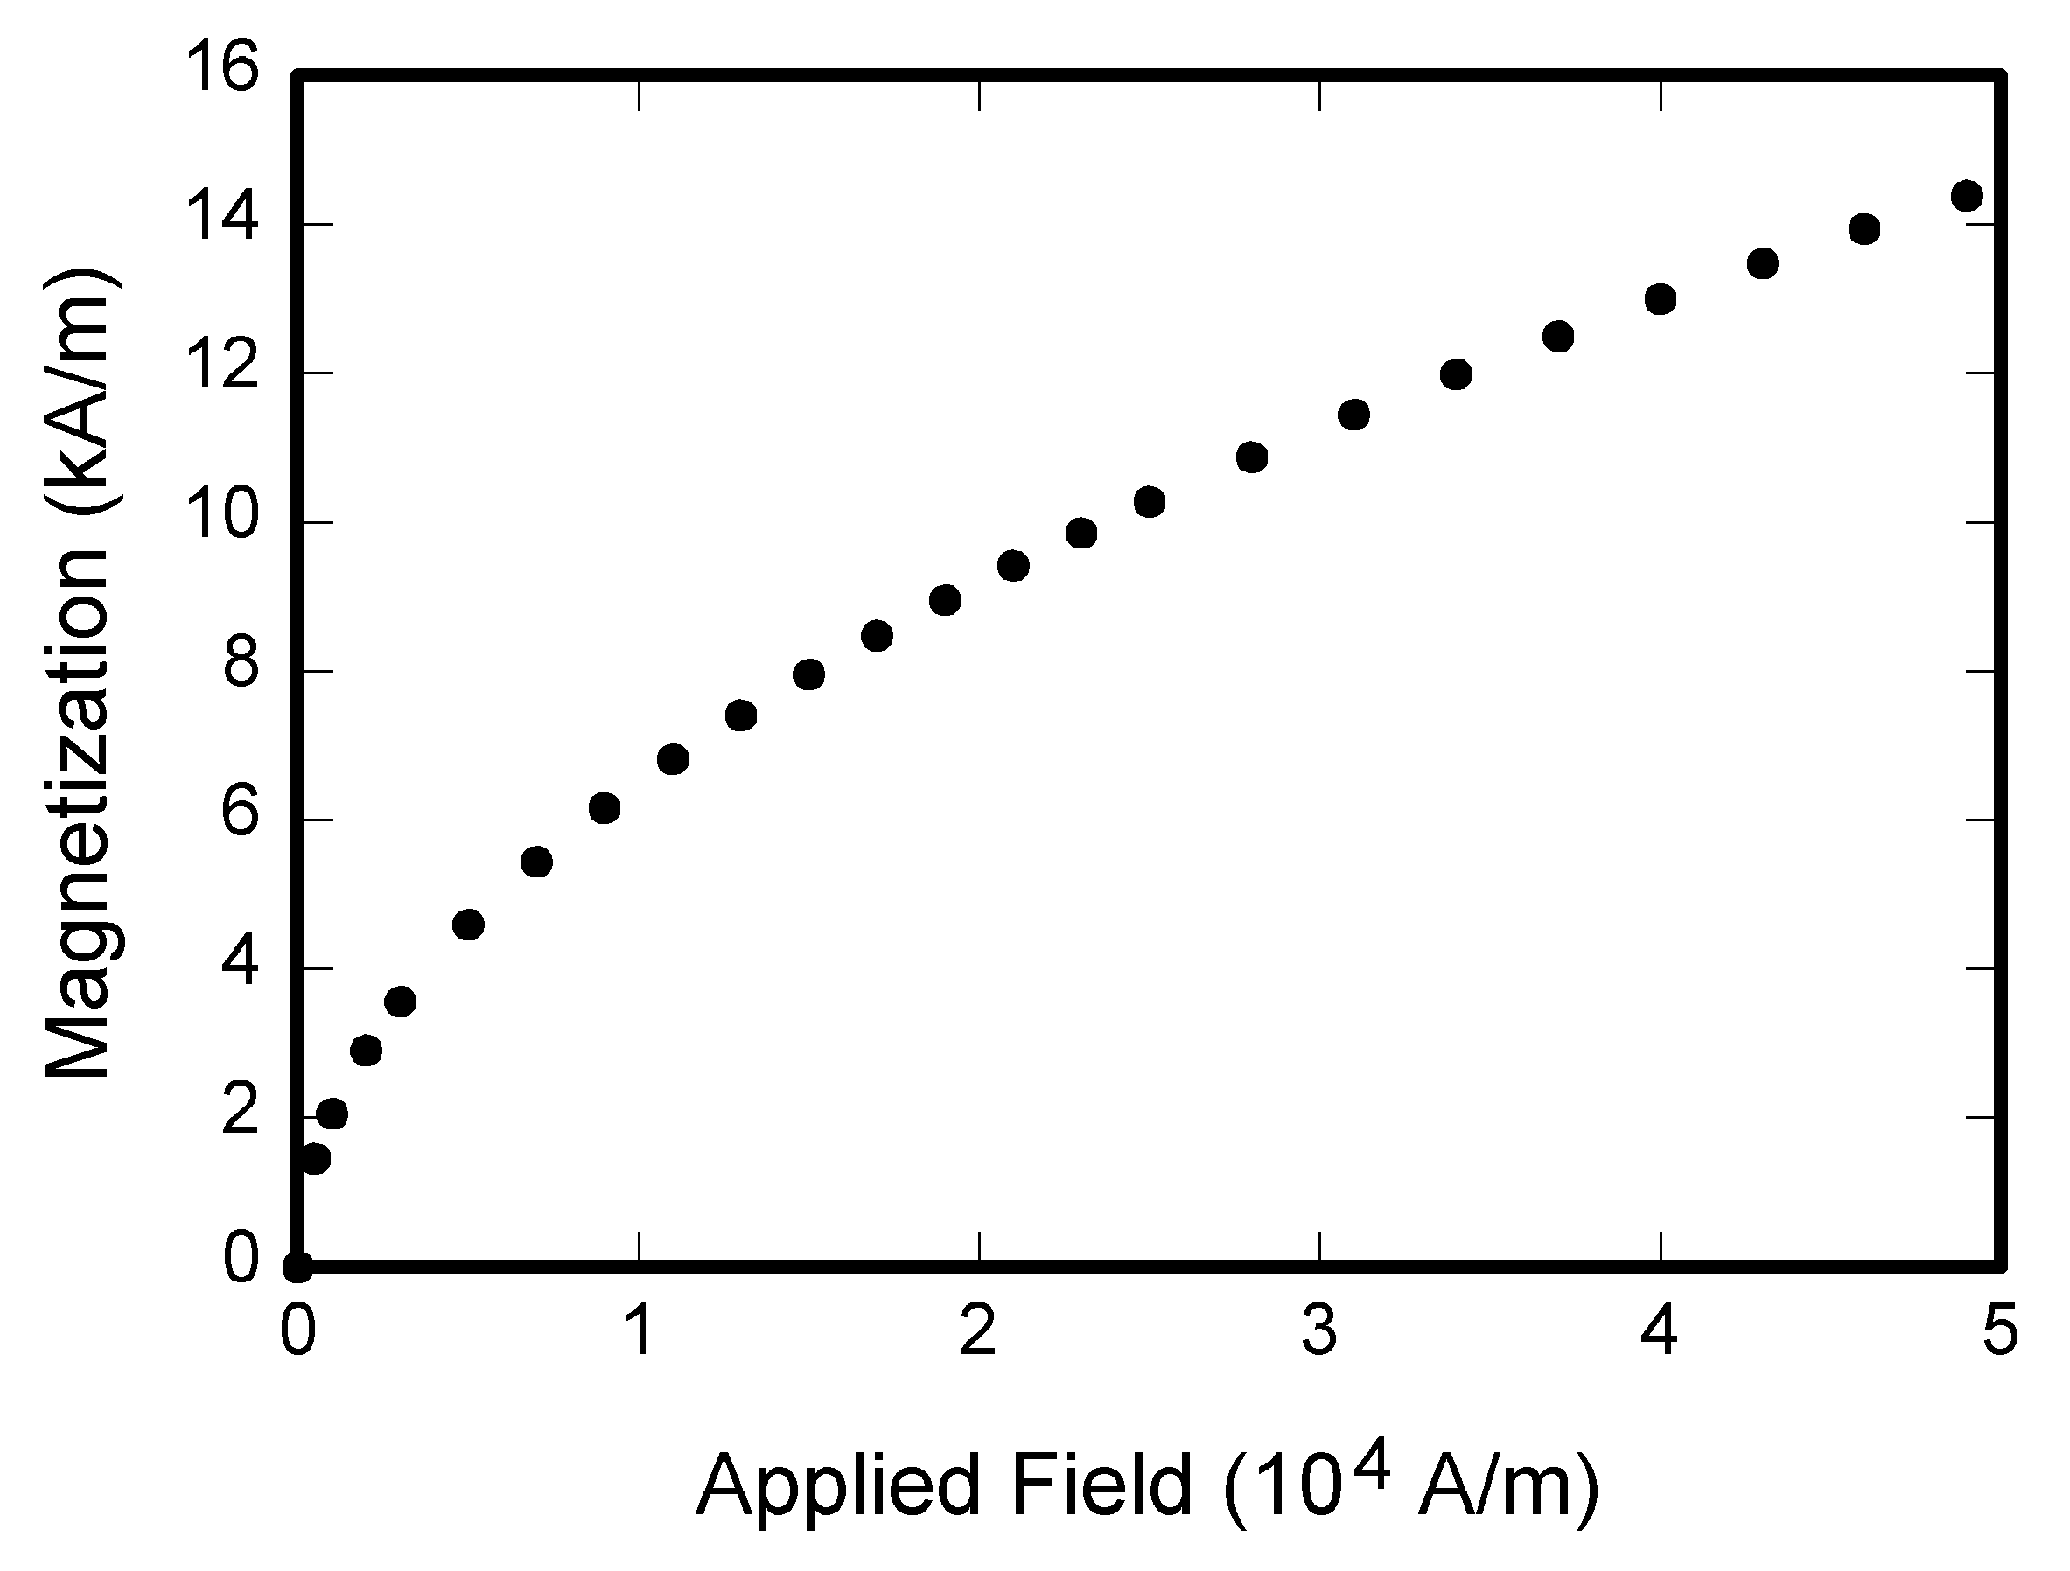
\includegraphics[width=\linewidth]{./fig1.png}
	\caption{Magnetization as a function of applied field. Note that “Fig.” is abbreviated. There is a period after the figure number, followed by two spaces. It is good practice to explain the significance of the figure in the caption.}
	\label{fig:examplesinglefig}
\end{figure}


\begin{table}[ht]
	\begin{center}	
		\small
		\resizebox{1\columnwidth}{!}{
			\begin{tabular}{ m{0.15\columnwidth} >{\raggedleft}m{0.35\columnwidth} m{0.5\columnwidth} }	
				\multicolumn{3}{c}{\textsc{Units for Magnetic Properties}} \\
				\hhline{===}
				{Symbol} & {Quantity} & {Conversion from Gaussian and CGS EMU to SI$^{a}$} \\ 
				\hline
				$\Phi$ & magnetic flux & $1~Mx\rightarrow 10^{-8}~Wb= 10^{-8}~V\cdot~S$\\
				B & magnetic flux density, magnetic induction & $1~G\rightarrow 10^{-4}~T= 10^{-4}~Wb/m^{2}$ \\
				H & magnetic field strength & $1~Oe\rightarrow 10^{3}/(4\pi)~A/m$\\
				m & magnetic moment & $1~erg/G=1~emu\rightarrow10^{-3}~A\cdot~m^{2}=10^{-3}A/m$\\
				M & magnetization & $1~erg/(G\cdot~cm^{3})=1~emu/cm^{3}\rightarrow10^{3}~A/m$ \\
				4$\pi$M & magnetization & $1~G \rightarrow10^{3}/(4\pi)~A/m$\\
				$\sigma$ & specific magnetization & $1~erg/(G\dot~g)=1~emu/g \rightarrow1~A\cdot~m^{2}/kg$ \\
				j & magnetic dipole moment & $1~erg/G=1~emu \rightarrow4\pi\times10^{-10}~Wb\cdot~m$\\
				J & magnetic polarization & $1~erg/(G\cdot cm^{3})=1~emu/cm^{3} \rightarrow4\pi\times10^{-4}~T$\\
				$\chi,\kappa$ & susceptibility & $1 \rightarrow4\pi$\\
				$\chi_{\rho}$ & mass susceptibility & $1~cm^{3}/g\rightarrow4\pi\times10{-3}~m^{3}/kg$ \\
				$\mu$ & permeability & $1\rightarrow4~\pi\times10^{-7}~H/m=4\pi\times10{-7}~Wb/(A\cdot~m)$\\
				$\mu_{\rho}$ & relative permeability & $\mu\rightarrow\mu_{r}$ \\
				w,W & energy density & $1~erg/cm^{3} \rightarrow10^{-1}~J/m^{3}$\\
				N,D & demagnetizing factor & $1 \rightarrow1/(4\pi)$\\
				\hhline{===}
				
			\end{tabular}
		}
	\end{center}
	\caption{Vertical lines are optional in tables. Statements that serve as captions for the entire table do not need footnote letters. \\
		$^{a}$Gaussian units are the same as cg emu for magnetostatics; Mx = maxwell, G = gauss, Oe = oersted; Wb = weber, V = volt, s = second, T = tesla, m = meter, A = ampere, J = joule, kg = kilogram, H = henry.
	}
	\label{Exp}
\end{table}
\normalsize

\subsection{Using Labels Within Figures}	
\subsubsection{Figure Axis labels}
Figure axis labels are often a source of confusion. Use words rather than symbols. As an example, write the quantity "Magnetization," or "Magnetization M," not just "M." Put units in parentheses. Do not label axes only with units. As in Fig. 1, for example, write “Magnetization (A/m)” or “Magnetization (A m$^1$),” not just “A/m.” Do not label axes with a ratio of quantities and units. For example, write “Temperature (K),” not “Temperature/K.” 
Figure labels should be legible, approximately 8 to 10 point type.\\

\subsubsection{Subfigure Labels in Multipart Figures and Tables}
Multipart figures should be combined and labeled before final submission. Labels should appear centered below each subfigure in 8 point Times New Roman font in the format of (a) (b) (c). 

\subsection{Referencing a Figure or Table Within Your Paper}
When referencing your figures and tables within your paper, use the abbreviation “Fig.” even at the beginning of a sentence. Do not abbreviate “Table.” Tables should be numbered with Roman Numerals.

\subsection{Checking Your Figures: The IEEE Graphics Checker}
The IEEE Graphics Checker Tool enables authors to pre-screen their graphics for compliance with IEEE Transactions and Journals standards before submission. The online tool is located at \underline{http://graphicsqc.ieee.org/}. For more information on using the Graphics Checker Tool 
or any other graphics related topic, contact the IEEE Graphics Help Desk by e-mail at \underline{graphics@ieee.org}.


\section{MATERIALS AND METHODS }	
Materials and methods can be expanded upon in the Supplementary Materials, if necessary.\\

SUPPLEMENTARY MATERIAL\\
Supplementary materials are encouraged and a short summary of the content of the Supplementary Materials section will appear before the acknowledgment. Please use the Supplementary Materials template. If you have Supplementary Materials, please use this section to direct readers to the Supplementary Materials and give them a brief overview of what they can expect to find in the Supplementary Materials. \\


ACKNOWLEDGEMENT\\
Use the singular heading even if you have many acknowledgments. Avoid expressions such as “One of us (S.B.A.) would like to thank ... .” Instead, write “F. A. Author thanks ... .” In most cases, sponsor and financial support acknowledgments are placed in the unnumbered footnote on the first page, not here.


\subsection{References}

See the end of this document for formats and examples of common references. For a complete discussion of references and their formats, see “The IEEE Style Manual,” available as a PDF link off the  \underline{\textit{Author Digital Toolbox}} main page.

\subsection{Footnotes}
Number footnotes separately in superscripts\footnote{It is recommended that footnotes be avoided (except for the unnumbered footnote with the receipt date on the first page). Instead, try to integrate the footnote information into the text.}.  Place the actual footnote at the bottom of the column in which it is cited; do not put footnotes in the reference list (endnotes). Use letters for table footnotes (see Table I). 


\section{Submitting Your Paper for Review}

{
\subsection{Uploading the Document}
All submissions must be uploaded via ScholarOne Manuscripts. Include full mailing addresses and e-mail addresses of all authors when uploading a manuscript. In addition, designate one author as the “corresponding author.” This is the author to whom proofs of the paper will be sent. Proofs are sent to the corresponding author only.

\subsection{Review Stage Using ScholarOne$^{\tiny\textregistered}$ Manuscripts}
Contributions to IEEE OJEMB must be submitted electronically on IEEE’s on-line manuscript submission and peer-review system, ScholarOne$^{\tiny\textregistered}$ Manuscripts at \textit{http://mc.manuscriptcentral.com/embs-ieee}. First check if you have an existing account. If there is none, please create a new account. After logging in, go to your Author Center and click “Submit First Draft of a New Manuscript.” 
There are various steps to the submission process; you must complete all steps for a complete submission. At the end of each step you must click “Save and Continue”; just uploading the paper is not sufficient. After the last step, you should see a confirmation that the submission is complete. You should also receive an e-mail confirmation. For inquiries regarding the submission of your paper on ScholarOne Manuscripts, please contact oprs-support@ieee.org or call +1 732 465 5861.

\subsection{Final Stage Using ScholarOne Manuscripts}
Upon acceptance, you will receive an email with specific instructions regarding the submission of your final files.  To avoid any delays in publication, please be sure to follow these instructions.  Final submissions should include source files of your accepted manuscript, high quality graphic files, and a formatted pdf file.  If you have any questions regarding the final submission process, please contact the administrative contact for the journal. 
}

\section{Editorial Policy}
{
Do not publish “preliminary” data or results. The submitting author is responsible for obtaining agreement of all coauthors and any consent required from sponsors before submitting a paper. IEEE OJEMB strongly discourages courtesy authorship. It is the obligation of the authors to cite relevant prior work. IEEE OJEMB expects the main source of references be archival journal articles or books or thesis. Conference proceeding papers should be minimized since many are not undergoing rigorous peer reviews. 
At least two reviews are required for every paper submitted. Indecipherable English is a valid reason for rejection. There is a service available that will help you improve your English for a fee, and the link to that service can be found at \textit{http://www.ieee.org/web/publications/authors/transjnl/ index.html}. 
}

\section{Publication Principles}
{
	The two types of contents of that are published are; 1) peer-reviewed and 2) archival. IEEE OJEMB publishes scholarly articles of archival value as well as tutorial expositions and critical reviews of classical subjects and topics of current interest. 
	Authors should consider the following points:
	\begin{enumerate}
		\item Technical papers submitted for publication must advance the state of knowledge and must cite relevant prior work. 
		\item The length of a submitted paper should be commensurate with the importance, or appropriate to the complexity, of the work. 
		\item Authors must convince both peer reviewers and the editors of the scientific and technical merit of a paper; the standards of proof are higher when extraordinary or unexpected results are reported. 
		\item Because replication is required for scientific progress, papers submitted for publication must provide sufficient information to allow readers to perform similar experiments or calculations and use the reported results. Although not everything need be disclosed, a paper must contain new, useable, and fully described information. For example, a specimen’s chemical composition need not be reported if the main purpose of a paper is to introduce a new measurement technique. Authors should expect to be challenged by reviewers if the results are not supported by adequate data and critical details.
		\item Papers that describe ongoing work or announce the latest technical achievement, which are suitable for presentation at a professional conference, may not be appropriate for publication.
	\end{enumerate}
	
	
}

\begin{thebibliography}{1}
	%\textit{Basic Format for Books:}\\
	\bibitem{BasicBook} \textbf{Basic Format for Books:} J. K. Author, Title of chapter in the book, in \textit{Title of His Published Book}, xth ed. City of Publisher, Country if not USA: Abbrev. of Publisher, year, ch. x, sec. x, pp. xxx–xxx.
	
	\bibitem{ExampleBook1} \textit{Example Book 1:} G. O. Young, “Synthetic structure of industrial plastics”, in \textit{Plastics},  2nd  ed.,  vol.  3,  J.  Peters,  Ed.  New  York: McGraw-Hill, 1964, pp. 15–64.
	
	\bibitem{ExampleBook2} \textit{Example Book 2:} W.-K. Chen, \textit{Linear Networks and Systems}. Belmont, CA: Wadsworth, 1993, pp. 123–135.\\
	
	\bibitem{BasicPeriodical} \textbf{Basic Format for Periodicals:} J. K. Author, “Name of paper”, \textit{Abbrev. Title of Periodical},  vol. x, no. x, pp. xxx-xxx, Abbrev. Month, year.
	
	\bibitem{ExamplePeriodical1} \textit{Example Periodical 1:} J. U. Duncombe, “Infrared navigation—Part I: An assessment of feasibility”, \textit{IEEE Trans. Electron Devices}, vol. ED-11, no. 1, pp. 34–39, Jan. 1959.
	
	\bibitem{ExamplePeriodical2} \textit{Example Periodical 2:} E. P. Wigner, “Theory of traveling-wave optical laser”, \textit{Phys. Rev.}, vol. 134, pp. A635–A646, Dec. 1965.
	
	\bibitem{ExamplePeriodical3} \textit{Example Periodical 3:} E. H. Miller et al., “A note on reflector arrays”,\textit{ IEEE Trans. Antennas Propagat.}, to be published.\\
	
	\bibitem{BasicHandbook} \textbf{Basic Format for Handbooks:} \textit{Name of Manual/Handbook}, x ed., Abbrev. Name of Co., City of Co., Abbrev. State, year, pp. xxx-xxx.
	
	\bibitem{ExampleHandbook1} \textit{Example Handbook 1:} \textit{Transmission Systems for Communications}, 3rd ed., Western Electric Co., Winston-Salem, NC, 1985, pp. 44–60.
	
	\bibitem{ExampleHandbook2} \textit{Example Handbook 2:} \textit{Motorola Semiconductor Data Manual}, Motorola Semiconductor Products Inc., Phoenix, AZ, 1989.\\
	
	\bibitem{BasicBookOnline} \textbf{Basic Format for Books (when available online):} Author. (year, month day). \textit{Title}. (edition) [Type of medium]. volume (issue). Available: site/path/file
	
	\bibitem{ExampleBookOnline} \textit{Example Book Available Online 1:} J. Jones. (1991, May 10). \textit{Networks}. (2nd ed.) [Online]. Available: http://www.atm.com\\
	
	\bibitem{BasicJournalOnline} \textbf{Basic Format for Journals (when available online):} Author. (year, month). Title. \textit{Journal}. [Type of medium]. volume (issue), pages. Available: site/path/file 
	
	\bibitem{ExampleJournalOnline} \textit{Example Journal Available Online 1:} R. J. Vidmar. (1992,  Aug.).  On  the  use  of  atmospheric plasmas as electromagnetic reflectors. \textit{IEEE Trans. Plasma Sci.} [Online]. 21(3), pp. 876–880. Available: http://www.halcyon.com/pub/journals/21ps03-vidmar\\
	
	\bibitem{BasicConferenceOnline} \textbf{Basic Format for Papers Presented at Conferences(when available online):} Author. (year, month). Title. Presented at Conference title. [Type of Medium]. Available: site/path/file
	
	\bibitem{ExampleConferenceOnline} \textit{Example Conference Paper Available Online 1:} PROCESS  Corp.,  MA.  Intranets:  Internet  technologies deployed behind the firewall for corporate productivity. Presented at 
	INET96 Annual Meeting. [Online]. Available:  http://home.process.com/Intranets/wp2.htp\\
	
	\bibitem{BasicReportsOnline} \textbf{Basic Format for Reports and Handbooks (when available online):} Author.   (year,   month).   Title. Company . City, State or Country. [Type of Medium]. Available: site/path/file
	
	\bibitem{ExampleReportOnline} \textit{Example Report Available Online 1:}  S.L.Talleen. (1996, Apr.). The Intranet  Architecture:  Managing  information  in  the  new paradigm. Amdahl Corp., CA. [Online]. Available: http://www.amdahl.com/doc/products/bsg/intra/infra/html\\
	
	 \textbf{Basic Format for Computer Programs and Electronic Documents (when available online):} ISO recommends that capitalization follow the accepted practice for the language or script in which the information is given.
	
	\bibitem{ExampleProgramOnline}\textit{Example Program Available Online 1:} A. Harriman. (1993, June). Compendium of genealogical software. \textit{Humanist}. [Online]. Available e-mail: HUMANIST@NYVM.ORG Message: get GENEALOGY REPORT\\
	
	\bibitem{BasicPatentsOnline} \textbf{Basic Format for Patents (when available online):} Name of the invention, by inventor’s name. (year, month day). \textit{Patent Number} [Type of medium]. Available: site/path/file\\
	
	\bibitem{ExamplePatentOnline}\text{Example Patent Available Online 1:} Musical toothbrush with adjustable neck and mirror, by L.M.R. Brooks. (1992, May 19). \textit{Patent D326189} [Online]. Available: NEXIS Library: LEXPAT File: DESIGN
	
	\bibitem{BasicConferencePublished} \textbf{Basic Format for Conference Proceedings (published):} J. K. Author, “Title of paper”, in \textit{Abbreviated Name of Conf.}, City of Conf., Abbrev. State (if given), year, pp. xxxxxx.

	\bibitem{ExampleBasicConferencePublished} \textbf{Basic Format for Conference Proceedings (published):} D. B. Payne and J. R. Stern, , “Wavelength-switched pas- sively coupled single-mode optical network,” , in \textit{in Proc. IOOC-ECOC}, 1985, pp. 585–590.

	\bibitem{BasicConferenceUnpublished} \textbf{Example for papers presented at conferences (unpublished):} 	D. Ebehard and E. Voges, “Digital single sideband detection for interferometric sensors”, presented at the 2nd Int. Conf. Optical Fiber Sensors, Stuttgart, Germany, Jan. 2-5, 1984.
	
	\bibitem{BasicFormatPatents} \textbf{Basic format for patents:} J. K. Author, J. K. Author, “Title of patent,” U.S. Patent x xxx xxx, Abbrev. Month, day, year.

	\bibitem{ExampleBasicFormatPatents} \textbf{Example Basic format for patents:} G. Brandli and M. Dick, “Alternating current fed power supply,” 
U.S. Patent 4 084 217, Nov. 4, 1978.


\end{thebibliography}


\end{document}